\documentclass[border=15pt, multi, tikz]{standalone}

\usepackage{tikz}
\usetikzlibrary{quotes,arrows.meta}
\usetikzlibrary{positioning}
\def\edgecolor{rgb:blue,4;red,1;green,4;black,3}
\newcommand{\midarrow}{\tikz \draw[-Stealth,line width =0.8mm,draw=\edgecolor] (-0.3,0) -- ++(0.3,0);}
\usepackage{Box}
\usepackage{RightBandedBoxNoBand}

\def\ConvColor{rgb:blue,5;green,2.5;white,5}
\def\ConvReluColor{rgb:blue,5;green,5;white,5}
\def\PoolColor{rgb:red,1;black,0.3}
\def\DcnvColor{rgb:blue,5;green,2.5;white,5}
\def\UnpoolColor{rgb:yellow,5;red,2.5;white,5}
\def\SoftmaxColor{rgb:magenta,5;black,7}

%\usetikzlibrary{3d} %for including external image 
\usepackage{tikz-3dplot}

\tikzset{
    axis/.style={-stealth,line width=2pt,every node/.append style={text=black}},
    xaxis/.style={axis,blue},
    yaxis/.style={axis,blue},
    zaxis/.style={axis,blue},
    xxaxis/.style={axis,green},
    yyaxis/.style={axis,green},
    zzaxis/.style={axis,green},
    bias/.style={axis,black,dashed,line width=0.6pt},
}


\begin{document}
\tdplotsetmaincoords{70}{115}
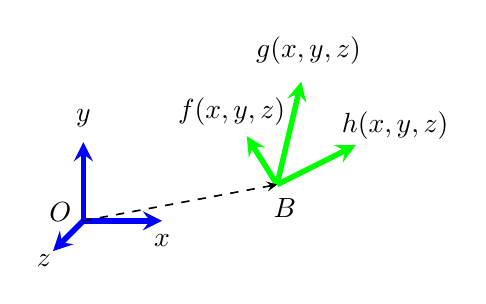
\begin{tikzpicture}

\node (label_O) at (-0.1,0.3,0.5) {$O$};
\node (label_B) at (4.1,1.7,4) {$B$};
\node (label_) at (0.5,0.5,0.5) {};
\draw[xaxis] (0,0,0) -- (1,0,0);
\node (label_x) at (1,-0.25,0) {$x$};
\draw[yaxis] (0,0,0) -- (0,1,0) node[pos=1.3]{$y$};
\draw[zaxis] (0,0,0) -- (0,0,1) node[pos=1.3]{$z$};

\draw[yyaxis] (4,2,4) -- (4,3,5)       node[pos=1.5]{$f(x,y,z)$};
\draw[zzaxis] (4,2,4) -- (4.5,3.5,4.5) node[pos=1.3]{$g(x,y,z)$};
\draw[xxaxis] (4,2,4) -- (5,2.5,4)     node[pos=1.5]{$h(x,y,z)$};

\draw[bias] (0,0,0) -- (4,2,4);

%\draw[dashed,->,>=stealth] (label_) to (label_B);

\end{tikzpicture}
\end{document}



